%%%% Proceedings format for most of ACM conferences (with the exceptions listed below) and all ICPS volumes.
\documentclass[sigconf]{acmart}
%%%% As of March 2017, [siggraph] is no longer used. Please use sigconf (above) for SIGGRAPH conferences.

%%%% Proceedings format for SIGPLAN conferences 
% \documentclass[sigplan, anonymous, review]{acmart}

%%%% Proceedings format for SIGCHI conferences
% \documentclass[sigchi, review]{acmart}

%%%% To use the SIGCHI extended abstract template, please visit
% https://www.overleaf.com/read/zzzfqvkmrfzn


\usepackage{booktabs} % For formal tables


% Copyright
%\setcopyright{none}
%\setcopyright{acmcopyright}
%\setcopyright{acmlicensed}
\setcopyright{rightsretained}
%\setcopyright{usgov}
%\setcopyright{usgovmixed}
%\setcopyright{cagov}
%\setcopyright{cagovmixed}


% DOI
\acmDOI{10.475/123_4}

% ISBN
\acmISBN{123-4567-24-567/08/06}

%Conference
\acmConference[GECCO '18]{the Genetic and Evolutionary Computation Conference 2018}{July 15--19, 2018}{Kyoto, Japan}
\acmYear{2018}
\copyrightyear{2018}


\acmArticle{4}
\acmPrice{15.00}

% These commands are optional
%\acmBooktitle{Transactions of the ACM Woodstock conference}
%\editor{Jennifer B. Sartor}
%\editor{Theo D'Hondt}
%\editor{Wolfgang De Meuter}


\begin{document}
\title{Understanding Evolutionary Computation with Ecological Theory}
%\titlenote{Produces the permission block, and
%  copyright information}
%\subtitle{}
%\subtitlenote{The full version of the author's %guide is available as
  %\texttt{acmart.pdf} document}


\author{Emily Dolson}
%\authornote{}
\orcid{0000-0001-8616-4898}
\affiliation{%
  \institution{BEACON Center for the Study of Evolution in Action, Department of Computer Science and Engineering, Program in Ecology, Evolutionary Biology and Behavior, Michigan State University}
  \streetaddress{567 Wilson Road Room 1441}
  \city{East Lansing} 
  \state{Michigan} 
  \postcode{48823}
}
\email{dolsonem@msu.edu}

\author{Charles Ofria}
%\authornote{}
\orcid{0000-0003-2924-1732}
\affiliation{%
  \institution{BEACON Center for the Study of Evolution in Action, Department of Computer Science and Engineering, Program in Ecology, Evolutionary Biology and Behavior, Michigan State University}
  \streetaddress{567 Wilson Road Room 1441}
  \city{East Lansing} 
  \state{Michigan} 
  \postcode{48823}
}
\email{ofria@msu.edu}


% The default list of authors is too long for headers.
\renewcommand{\shortauthors}{E. Dolson and C. Ofria}


\begin{abstract}
Evolutionary algorithms often incorporate ecological concepts to help maintain diverse populations and drive continued innovation. However, while there is strong evidence for the value of ecological dynamics, the precise mechanisms behind these results are not always clear. These gaps in our understanding make it challenging to predict which approaches will be most appropriate for a given problem. Ecologists have addressed similar questions for many decades, but the resulting body of theory has yet to be fully translated into an evolutionary context. This paper lays the groundwork for such a translation by adapting ecological theory to three different selection mechanisms in evolutionary computation: fitness sharing, lexicase selection, and Eco-EA. First, we use ecological ideas to establish a framework that clarifies where these selection schemes are alike and where they differ. We then build upon this framework by using metrics from ecology to gather empirical data about the underlying differences in the population dynamics that these approaches produce. Specifically, we measure phylogenetic relationships within the population to explore long-term stable coexistence. These results can inform parameter selection, choice of selection scheme, and the development of new selection schemes.

\end{abstract}

%
% The code below should be generated by the tool at
% http://dl.acm.org/ccs.cfm
% Please copy and paste the code instead of the example below. 
%
\begin{CCSXML}
<ccs2012>
<concept>
<concept_id>10010147.10010257.10010293.10011809.10011810</concept_id>
<concept_desc>Computing methodologies~Artificial life</concept_desc>
<concept_significance>500</concept_significance>
</concept>
<concept>
<concept_id>10010147.10010257.10010293.10011809.10011812</concept_id>
<concept_desc>Computing methodologies~Genetic algorithms</concept_desc>
<concept_significance>500</concept_significance>
</concept>
<concept>
<concept_id>10010147.10010257.10010293.10011809.10011813</concept_id>
<concept_desc>Computing methodologies~Genetic programming</concept_desc>
<concept_significance>500</concept_significance>
</concept>
</ccs2012>
\end{CCSXML}

\ccsdesc[500]{Computing methodologies~Artificial life}
\ccsdesc[500]{Computing methodologies~Genetic algorithms}
\ccsdesc[500]{Computing methodologies~Genetic programming}


\keywords{Diversity, diversity maintenance, fitness sharing, lexicase selection, Eco-EA, ecology, ecological theory, eco-evolutionary dynamics, phylogenetic analysis}


\maketitle

\section{Introduction}

Evolutionary computation researchers have devoted a great deal of attention to understanding how to promote stable coexistence between lineages exploring different regions of a fitness landscape~\cite{goldberg_genetic_1987,mahfoud_niching_1995, mouret_using_2009,pugh_confronting_2015}. Promoting diversity within an evolving population is important for evolutionary computation because it encourages exploration of a higher percentage of the fitness landscape and reduces the chances of premature convergence on a suboptimal fitness peak. However, some types of diversity facilitate finding the global optimum better than other types. For instance, increasing the mutation rate generates more new genotypes but is unlikely to meaningfully increase the spread of the population across the fitness landscape. Even amongst more advanced approaches to generating and maintaining diversity, some seem to systematically produce diversity that is spread across the fitness landscape in ways that are more conducive to solving a given problem than the diversity produced by other approaches (see, for instance, the difference between the probe and behavioral methods in~\cite{mouret_using_2009}, or the different evolutionary potential observed at equivalent diversity levels in~\cite{walker_evolutionary_2012}). In most cases, we have a high-level idea of why a given technique promotes diversity, but uncertainty remains about the mechanistic details that lead to it being spread across the fitness landscape in different ways. For example, we know that fitness sharing~\cite{goldberg_genetic_1987} promotes diversity via negative density dependence. Is this diversity spread across the fitness landscape differently from diversity promoted by, for instance, lexicase selection~\cite{spector_assessment_2012}? The answer to this question depends on subtle differences in the evolutionary pressures that these different selection schemes place on the evolving population, which have yet to be fully untangled.

Because techniques for promoting diversity rely on creating interactions  between individuals in the population (other than the default equal competition for space with all other population members), they are, by definition, creating simple ecologies. Ecologists have developed rigorous theory to predict how ecological communities will change over time. In particular, they have done a great deal of research on the conditions under which long term stable coexistence between different ecotypes is possible~\cite{pacala_limiting_1994, chesson_mechanisms_2000,chase_ecological_2003,letten_linking_2017}. Predicting when stable coexistence will occur in evolutionary computation allows us to determine which pathways through a fitness landscape can simultaneously be traversed by a given evolutionary algorithm, a critical component of predicting which approach will be most effective in a given scenario. This insight should apply both to choosing an appropriate diversity maintenance technique and to choosing appropriate parameters for it. Additionally, an improved mechanistic understanding of why existing algorithms work should facilitate building more effective variations on those algorithms.

There are two main sets of tools from ecology that we expect will be helpful to analyzing evolving communities in evolutionary computation: mathematical theory and empirical measurements. Mathematical theory is useful for making \textit{a priori} predictions about the outcome of various evolutionary set-ups, however it can be challenging to translate into the realm of evolutionary computation. Doing so requires careful attention to implicit assumptions about nature that may not translate to a computational population. A more substantial problem is that most ecological theory assumes that the population is not evolving fast enough to be relevant (although recent research on eco-evolutionary dynamics has begun to bridge this gap). Attempting to introduce evolution can create messy feedback loops. Another important limitation to keep in mind is that equations in ecology generally calculate the average or expected behavior of a system. This can be misleading in highly stochastic processes, such as evolution. Nonetheless, mathematical theory is a useful starting point for predictions. As such, we will lay some groundwork here for using it to guide development of evolutionary computation systems.

Empirical measurements are an important complementary approach to mathematical theory. Where the latter can be used to make predictions, the former can be used to assess the accuracy of these predictions. Even in cases where we do not have a math-based prediction, we can use empirical measurements to uncover general patterns. Ecologists have developed a broad toolbox of ways to quantify various aspects of an ecological community. Among these tools are a suite of measurements for evaluating the diversity of the community. Some of these metrics, such as richness (number of unique ecotypes) and Shannon diversity have already made their way into common usage in evolutionary computation. Others, however, such as various measurements of phylogenetic diversity~\cite{winter_phylogenetic_2013}, have yet to do so. Phylogenetic diversity in particular has the potential to offer useful insights in the context of evolutionary computation, as it can assess the extent to which an algorithm is producing deep phylogenetic branches that explore distinct parts of the fitness landscape vs. ecotypically varied individuals that only recently diverged from a common ancestor. This distinction is an example of the sort that is likely to have implications for how usefully the population is spread across the fitness landscape. We can also use empirical ecological measurements to assess hypothesized mechanisms about why different diversity maintenance techniques have different effects. Since an ecological community is just a group of individuals that interact with each other in various ways, ecologists often build graphs representing the interactions between community members. The topology of these graphs has various implications for the way the community will change over time~\cite{fontaine_ecological_2011}. We can do the same for communities in evolutionary computation.

In the rest of this section, we will provide a little bit more background on ecological theory and the selection schemes that we'll be exploring with it. In the rest of this paper, we will explore what this framework can tell us about evolutionary computation and lay the groundwork for easier application of ecological ideas to evolutionary computation in the future.

\subsection{Ecological theory}

While a lot of ecological theory is potentially useful to understanding evolutionary computation, the most obviously critical connections relate to the circumstances under which different types of organisms can or cannot coexist with each other. If we can predict when coexistence is or is not possible within a given evolutionary algorithm, we will have a window onto the types of lineages that can simultaneously explore the fitness landscape. Thus, determining coexistence criteria will be the primary focus of this paper. Conveniently, this issue is also of central importance to ecologists.

Initial work on coexistence in ecology focused on competition for resources that are both \textit{limited} in quantity, and \textit{limiting} in the sense that they determine the rate of growth of the competing species. The most important value for determining coexistence in this context is a species' $R^{*}$, the resource availability level at which the species' growth rate is 0. In the simplest case, where species are competing for a single resource, the species with the lowest $R^*$ for that resource should out-compete the others~\cite{grover_resource_1997}. That species' population will continue to increase, depleting the resource until it reaches the species' $R^*$; meanwhile, the resource availability will dip below the other species' $R^*$, causing their populations to decrease. Adding additional resources introduces the potential for stable coexistence between multiple species, if each species is a better competitor for a different resource and consumes more of that resource~\cite{chase_ecological_2003}, summarized in~\cite{letten_linking_2017}). 

This is a specific instance of a much broader rule: species can coexist if each species competes with itself more than it competes with the other species~\cite{chesson_mechanisms_2000}. This rule works because it forces species to be self-limiting, creating negative frequency dependent dynamics where each additional member of a species reduces that species' growth rate~\cite{adler_niche_2007}. The magnitude of difference between inter- and intra-specific competition that is required to enable long-term stable coexistence is determined by the difference in the fitness of the two species. If one species is dramatically more fit, it can drive the other to extinction even if they only compete to a small extent~\cite{chesson_mechanisms_2000}. Ecologists draw a distinction between "stabilizing" dynamics, which alter the ratio of interspecific competition and intraspecific competition, and "equalizing dynamics" which alter the difference in fitness between two species~\cite{adler_niche_2007}. Note that in biology, "fitness" refers strictly to reproductive output, rather than the externally-defined "fitness functions" used in evolutionary computation. Thus, approaches such as Hierarchical Fair Competition~\cite{hu_hierarchical_2005} and Age-Layered Population Structures~\cite{hornby_alps:_2006}, which give additional offspring to low-fitness individuals without adjusting their fitness as the defined by the fitness function, would be examples of equalizing dynamics. The critical difference between stabilizing and equalizing dynamics is that, in the absence of any stabilizing dynamics, equalizing dynamics lead to an unstable equilibrium; even if two species have identical fitness, drift should eventually lead to one going extinct. Stabilizing dynamics, on the other hand, actively correct any deviation from the equilibrium populations of each species.

The research discussed so far has made the assumption that competing species inhabit the same physical region and are competing to harvest resources from that region. If we consider a broader spatial region, however, there is another mechanism for coexistence: instead of using different resources, different species might live in different parts of the environment. This form of coexistence is most intuitive if there are harsh abiotic conditions that must be overcome in order to survive somewhere. For instance, living in one corner of the world might require tolerance to extreme heat, while another region might require tolerance to acidic soil. In this case, species would only compete with other species that could inhabit some of the same regions.

What does all of this mean for evolutionary computation? First, when choosing parameters, we should consider the circumstances under which they promote coexistence; when two independent lineages are traversing the fitness landscape, how close to each other can they pass without risking one going extinct? In section 2, we will address this question in the contexts of some specific algorithms. Second, when designing selection schemes, we should determine how costly it is to stochastically lose lineages from the population. If it is costly, we should consider including stabilizing dynamics in addition to or in place of equalizing dynamics. Lastly, we should give careful thought to the metaphors that we use to compare evolutionary computation to biological populations; determining whether a given selection scheme is more akin to competition for resources, spatially segregated habitats, or something else all-together will make it much easier to draw parallels. If we can show that a system in evolutionary computation is isomorphic to a system in biology, we can rapidly import insights from the biological research into how that system behaves.

\subsection{Empirical ecological techniques}

The central challenge in empirical ecology is attempting to find general patterns  from complex, messy data. While data in evolutionary computation may be less messy than ecological field data, the interconnections within any ecological community are complex. Ecologists have come up with many tools for extracting meaning out of this complexity, which may be equally helpful to those trying to understand the fine-scale dynamics of evolutionary computation algorithms. Here we will focus on two approaches: phylogenetic analysis and interaction networks.

\subsubsection{Phylogenetic analysis}
Phylogenetic analysis refers to a suite of metrics that can be used to summarize the topology of the populations' phylogeny (ancestry tree)~\cite{winter_phylogenetic_2013}. In biology, these trees generally need to be inferred from extant species, but in evolutionary computation we have the advantage of perfect phylogenetic knowledge. Many of these methods are focused around inferring the amount of evolutionary history that a current population contains. For instance, a population with with members from branches that have been evolving independently for a long time contains more evolutionary history than a population that is all descended from a recent common ancestor. Even if the latter population contains many unique phenotypes, they are all relatively close to each other on the fitness landscape. These means that A) they could be easily regenerated if some were lost, and B) the population is most likely not exploring multiple basins of attraction within the fitness landscape, which is usually the goal of diversity maintenance techniques. For this reason, phylogenetic diversity provides information about the efficacy of a diversity maintenance technique above and beyond the more commonly used measures of genotypic and phenotypic diversity.

Techniques for analyzing the topology of phylogenies can be split into three categories: richness (total quantity of evolutionary history represented), divergence (how spread out the population is in phylogenetic space), and regularity (how evenly is the population divided across evolutionary space)~\cite{tucker_guide_2017}. For the purposes of this paper, we will focus on richness and divergence, as our goal here is to analyze selection schemes and we suspect that regularity has more to do with the search space. However, regularity has the potential to be a powerful tool for analyzing the fitness landscape as it is being explored and is worthy of future study. A number of metrics exist for measuring both phylogenetic richness and phylogenetic divergence (summarized in~\cite{winter_phylogenetic_2013} and~\cite{tucker_guide_2017}). Here, we will measure phylogenetic richness with the original phylogenetic diversity metric (simpled referred to "phylogenetic diversity")~\cite{faith_conservation_1992},  which sums the lengths of the shortest path from each extant genotype to the most recent common ancestor. We will measure divergence as the mean pairwise distance between genotypes in the population~\cite{webb_exploring_2000}.  

Note that in biology, there is an implicit assumption that the root of the tree is the most recent common ancestor of all taxonomic units being compared. In the context of biology this is obvious, because phylogeny reconstruction techniques cannot make inferences about anything preceding the most recent common ancestor. In evolutionary computation, however, we have the full history, and so it is worth stating explicitly that we excluding history before the most recent common ancestor. Including this history would not add any additional information; it would increase phylogenetic diversity by a constant amount for each member of the population and leave mean pairwise distance unchanged. Note also that we chose here to calculate these metrics on a per-genotype basis, but could just as easily have calculated them per-individual or per-phenotype.

\subsubsection{Interaction networks}
Since ecological communities are collections of organisms interacting with each other, a useful technique for understanding them is to draw a graph representing the network of interactions. The topology of this graph can help us to understand the selective pressures that organisms are placing on each other. In ecology, these networks are often generated from knowledge of the species involved as a proxy for fitness information. For instance, if two species use the same limited resource, then they must compete with each other. As was the case with phylogenies, in evolutionary computation there's an easier way: we can directly measure the fitness of each member of the population with and without each other member present and compare the difference.
%should probably say more here? and have citations.

\subsection{Selection schemes}

For the purposes of this paper, we have chosen a subset of selection schemes from the vast range of diversity maintenance techniques. Specifically, we have selected the approaches that most clearly map onto ecology. In the future, we hope to expand this framework to include a wider variety of diversity maintenance techniques. In the remainder of this paper, we will explore the ecological communities generated by these approaches. For those who are not familiar with the selection schemes we have chosen, we offer a capsule summary of each.

\subsubsection{FItness sharing}

Fitness sharing was one of the first uses of ecology to promote diversity in evolutionary computation~\cite{goldberg_genetic_1987}. In fitness sharing, the fitness of every member of the population is reduced in proportion to the number of similar individuals (i.e. they "share" their fitness). Specifically, the number of other occupants of a niche is calculated by summing the sharing equation, $sh(d)$, over the population:

\begin{equation} sh(d) =    \begin{cases}
      1 - (\frac{d}{\sigma_{share}})^{\alpha} & d < \sigma_{share}\\
      0 &  d \geq \sigma_{share}  
   \end{cases}
\label{eq:fit_share}
\end{equation}
where $d$ is the distance between the individual that is currently having its fitness calculated and another member of the population. This distance can be defined in terms of genotype or phenotype.  Each organism's fitness is then divided by the sum of the sharing equation.

\subsubsection{Lexicase selection}

In lexicase selection, a large number of criteria are chosen for solutions to be evaluated on~\cite{spector_assessment_2012}. Traditionally, these criteria are each individual test cases, but recent work suggests that other types of fitness functions are also effective [CITE GPTP paper?]. Every time an individual is selected to reproduce, the selection criteria are randomly reordered. The entire population is evaluated on the first one. The individuals that perform best on this first criterion are then evaluated on the second criterion. The ones that perform best on that criterion are then evaluated on the third, and so on, until only one individual remains or all criteria have been used and the winner is selected randomly from the remaining options.

Lexicase selection has proven to be highly effective at solving challenging problems in genetic programming~\cite{helmuth_general_2015,helmuth_solving_2015} and maintaining diverse populations while doing so~\cite{helmuth_effects_2016}. Prior work on the population dynamics of lexicase selection has largely centered around the surprising prevalence of "hyperselection events," occasions on which a single individual was selected as a parent for a very high percentage of the next generation~\cite{mcphee_using_2016}. Given lexicase selection's success at maintaining the diversity, the fact that such events occurred at all was surprising. Further research, however, has suggested that these events are not important an important part of of lexicase selection's success at solving challenging problems and maintaining diversity~\cite{helmuth_impact_2016}. Additional case studies of phylogenetic trees generated by lexicase selection are consistent with the idea that lexicase selection promotes the existence of sub-populations that are focused on a specific selection criterion~\cite{mcphee_visualizing_2016}.

\subsubsection{MAP-Elites}

In MAP-Elites~\cite{mouret_illuminating_2015}, the user selects some number of dimensions along which they would like to see a diversity of solutions, and the search space defined by those dimensions is discretized into bins. Whenever a new individual is created, it is assessed on each dimension and put into the corresponding bin is located. If the bin is empty, or the individual currently occupying it has lower fitness than the newcomer, the newly created individual is placed into the bin, replacing any existing occupant. If the bin is already occupied by an individual with higher fitness than the new individual, the new individual is discarded. Not only has this approach proven effective at solving problems, particularly those where a variety of phenotypic options are desirable~\cite{cully_robots_2015}, it also provides insight intro trade-offs inherent in the search space.

\subsubsection{Eco-EA}

Developed by Goings and Ofria, Eco-EA is an approach to solving complex problems by associating limited resources with solving various sub-problems~\cite{goings_ecological_2009,goings_natural_2010,goings_ecology-based_2012}. Generally, these are simpler versions or components of the larger problem, but they could also be test cases, or other related tasks that are expected to be helpful to finding a global solution. Resources flow into the population at a constant rate, building up until a solution to the corresponding sub-problem is discovered. When a population first solves a sub-problem, the associated resource is plentiful so the individuals capable of using it are very successful. As the number of individuals using the resource increases, it become less valuable. The goal of this set-up is to use negative frequency dependence to create stable populations within the niche associated with each resource. However, full negative frequency dependence is only possible if there is a cost to attempting to use a resource. Without a cost, the benefit of using a resource diminishes as the number of individuals using it increases, but no individual's fitness can actually be reduced by trying and failing to use it. As a result, without a cost, there is no pressure to maintain diversity. Early work with Eco-EA featured problems with inherent tradeoffs, creating an implicit cost \cite{goings_ecological_2009,goings_ecology-based_2012}. When Eco-EA was extended to other problems without such tradeoffs, an explicit cost was introduced [cite GPTP paper].

%Eco-EA has proven to be effective at evolving diverse 

\section{Theory}

- Things to consider for each:
- biological fitness, w
- when can stable coexistence happen
- what is diversity with respect to/what are niches

\subsection{Fitness sharing}

cite Deb paper that already did all the math

\subsection{Lexicase selection}

In ecological terms, lexicase selection creates a vast number of niches nested within each other. While it is tempting to use a resource metaphor to understand the competition within these niches, this is actually incorrect and misleading. Whereas using a resource harms all other individuals that use that resource, improving on a selection criterion in lexicase selection only harms a (usually small) subset of the population. Instead, we argue that population structure is a better metaphor for lexicase selection. Imagine $N!$ islands, where $N$ is the number of selection criteria and each island corresponds to a single potential ordering of selection criteria and can only be inhabited by the individuals that are best at that ordering. Each island has a fixed amount of space. This is analogous to situations in nature where niches are defined exclusively by an organism's ability to survive a set of abiotic conditions. Being better able to survive these conditions increases the number of offspring an individual can have. Over time, genotypes that are better at surviving in a given set of conditions competitively exclude those that are worse at surviving there. In the case of lexicase selection, this competitive exclusion happens more rapidly than it usually would in biology, but the principle is the same. 

[Mention weird thing about all space being adjacent]
[note that subpopulations are consistent with observations from tree paper]

$N!$ is the maximum number of genotypes that should be able to stably coexist in the long term within a population under lexicase selection. While islands can potentially be inhabited by multiple genotypes that are equally able to occupy it, this coexistence will be unstable if neither genotype has another island to itself. The instability results from the fact that, within a single island, each genotype has equal fitness and competes with itself the same amount that it competes with other genotypes on the island. Thus, as stated in equation [EQUATION], there is no stabilizing pressure to increase the populations of rare genotypes within an island. Eventually, all but one should stochastically go extinct.

Because of the laws of probability, this coexistence is not technically permanent. Orderings are selected randomly, and there is always a chance that a given one will not be selected on a given generation. However, as the number of solutions that can live on each island ($\frac{population}{N!}$) increases, the odds of a catastrophic event that wipes out a whole island decrease rapidly. We can extend this rule to also cover the many cases where the total population size is less than the number of islands (i.e. islands can support less than one individual each). In these cases, it is no longer sufficient to control a single island. Instead, we calculate the sum of the total controlled area (counting fractions of islands, in the case of ties). This process produces a single number, $w$ for each genotype, indicating what fraction of the total space it controls. We use the variable $w$ here for consistency with biological theory, because this value also corresponds to an individual's probability of being selected, i.e. its biological fitness. Just as species in nature face greater risk of stochastic extinction of their range (the area they inhabit) is too small, so too do genotypes in lexicase selection. The chances of surviving for $G$ generations are given by the equation:

\begin{equation}
P(survival) = (1 - (1-w)^{population size})^{G}
\end{equation}
\begin{figure}
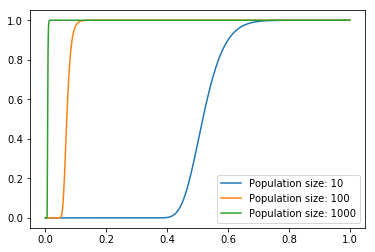
\includegraphics[width=1.5in]{figs/survival_pop_size.png}
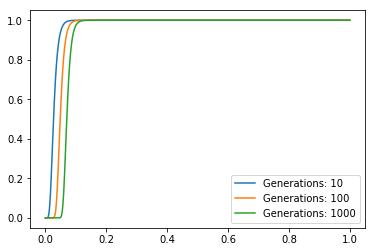
\includegraphics[width=1.5in]{figs/survival_generations.png}
\caption{}
\label{prob_survival}
\end{figure}

Plotting this function for various values of population size and $G$, we see that there is generally a cut-off value where the probability of survival rises abruptly from approximately 0 to approximately 1 (see Figure \ref{prob_survival}). In this way, we can effectively calculate the minimal size of the region a genotype must occupy in order to be likely to survive in the long term. This value is closely related to the concept of a minimum viable population in biology, and is useful to consider when making decisions about how large of a population size to use. 

From this analysis, we can conclude that lexicase selection produces 

The selection criteria determine which other individuals in the population a given solution is competeing with for space. 

\subsection{MAP-Elites}

The criteria for stable coexistence in MAP-Elites are refreshingly straightforward. Like lexicase selection, MAP-Elites can be thought of as an alternative population structure. Each location in the spatial structure can only be occupied by individuals that fall in the correct phenotypic range. Within a location, competitive exclusion happens immediately. Because each individual can only occupy one location in the population, there is no competition. All members of the population have equal biological fitness, $w$, and all are capable of stable coexistence for an infinite length of time (because individuals stay in the population until they are replaced, there isn't even a risk of stochastic extinction).

\subsection{Eco-EA}

At equilibrium, the amount of resource that each solution receives, $A_{i}$ should be equal to the rate at which the resource enters the environment, $I$, divided by the number of solutions using the resource, $N_{ui}$ [cite Sherri's thesis]. $R^{*}$, the lowest resource availability at which an individual can benefit from a resource, should be $\frac{cost}{C_{f}*score}$. Note that $R^{*}$ is lower for high scores, which is consistent with the biological metaphor. A new genotype that is better at the task associated with a resource would be able to invade the niche, because it would drive the amount of available resource down while still deriving benefit from using it, whereas the genotype with the higher $R^{*}$ would cease to derive a benefit. 

\section{Empirical Methods}

While theory offers a good mental framework to understand empirical results, it can easily get detached from reality. This is especially true in the case of systems with substantial stochasticity and feedback loops, such as evolutionary systems. In such situations, the average case predicted by theory may not actually be particularly representative. Thus, to strengthen our intuition for the ecology of these selection schemes, we will now investigate them in the context of actual populations. 

\subsection{Interaction networks}
In section 2, we made a number of predictions about the competitive pressures that different selection schemes exert on a population. We can assess the accuracy of these predictions by drawing interaction networks for populations being subjected to these selection schemes. For ease of understanding in the context of this preliminary analysis, we will use very simple populations. The individuals in these populations are vectors of 5 numbers. Each number represents a niche which these individuals are competing to occupy. In the context of fitness sharing, this means that distance is measured as euclidean distance between each pair of vectors. For lexicase selection, each position in the vector is a selection criterion and the individual with the highest value there wins. In Eco-EA, there is a resource associated with each position in the vector and an individual's value at that position defines its ability to use that resource. For simplicity, the fitness landscape is otherwise flat. We will compare the same population of 10 individuals across all selection schemes. To calculate the effect that a given individual, $A$ has on another individual, $B$, we first calculate the fitness of $A$ in the presence of the whole population. Then we remove $B$ from the population and recalculate the fitness of $A$. The difference between these two fitnesses is the effect of $A$ on $B$. Note that these fitness values are biological fitness, i.e. the probability of being selected to reproduce, rather than the fitness produced by the fitness function.  For fitness sharing and Eco-EA, we assumed a tournament size of 2 when making this calculation.

\subsection{Phylogenetic analysis of evolved populations}

\subsection{Statistical methods}


\subsection{Code availability}
Data for the interaction network analysis was generated using a simple simulation written with Python 3.6.3. Graphs were visualized using the networkx package~\cite{hagberg_exploring_2008}. The code for empirical analysis of evolved populations was written in C++ using the [REMOVED FOR DOUBLE-BLIND] library. Statistical analysis was performed using the R statistical computing language version 3.4.3~\cite{r_core_team_r:_2017} and graphs were made with the ggplot2 package~\cite{wickham_ggplot2:_2009}. All code for generating and analyzing the data presented in this paper is open source and available at [REMOVED FOR DOUBLE-BLIND]. 

\section{Results and Discussion}

\subsection{}

\section{Conclusions}

- Theory summary table

\begin{acks}
We extend our thanks to Alex Lalejini and Matthew Moreno for their helpful comments and suggestions on early drafts of this manuscript. This research has been supported by the National Science Foundation (NSF) BEACON Center under Cooperative Agreement DBI-0939454, by an NSF Graduate Research Fellowship to ED under Grant No. DGE-1424871, and by Michigan State University through computational resources provided by the Institute for Cyber-Enabled Research. Any opinions, findings, and conclusions or recommendations expressed in this material are those of the author(s) and do not necessarily reflect the views of the NSF.
\end{acks}


% \subsection{Citations}
% Citations to articles~\cite{bowman:reasoning,
% clark:pct, braams:babel, herlihy:methodology},
% conference proceedings~\cite{clark:pct} or maybe
% books \cite{Lamport:LaTeX, salas:calculus} listed
% in the Bibliography section of your
% article will occur throughout the text of your article.
% You should use BibTeX to automatically produce this bibliography;
% you simply need to insert one of several citation commands with
% a key of the item cited in the proper location in
% the \texttt{.tex} file~\cite{Lamport:LaTeX}.
% The key is a short reference you invent to uniquely
% identify each work; in this sample document, the key is
% the first author's surname and a
% word from the title.  This identifying key is included
% with each item in the \texttt{.bib} file for your article.

% The details of the construction of the \texttt{.bib} file
% are beyond the scope of this sample document, but more
% information can be found in the \textit{Author's Guide},
% and exhaustive details in the \textit{\LaTeX\ User's
% Guide} by Lamport~\shortcite{Lamport:LaTeX}.

% This article shows only the plainest form
% of the citation command, using \texttt{{\char'134}cite}.

% Some examples.  A paginated journal article \cite{Abril07}, an enumerated
% journal article \cite{Cohen07}, a reference to an entire issue \cite{JCohen96},
% a monograph (whole book) \cite{Kosiur01}, a monograph/whole book in a series (see 2a in spec. document)
% \cite{Harel79}, a divisible-book such as an anthology or compilation \cite{Editor00}
% followed by the same example, however we only output the series if the volume number is given
% \cite{Editor00a} (so Editor00a's series should NOT be present since it has no vol. no.),
% a chapter in a divisible book \cite{Spector90}, a chapter in a divisible book
% in a series \cite{Douglass98}, a multi-volume work as book \cite{Knuth97},
% an article in a proceedings (of a conference, symposium, workshop for example)
% (paginated proceedings article) \cite{Andler79}, a proceedings article
% with all possible elements \cite{Smith10}, an example of an enumerated
% proceedings article \cite{VanGundy07},
% an informally published work \cite{Harel78}, a doctoral dissertation \cite{Clarkson85},
% a master's thesis: \cite{anisi03}, an online document / world wide web
% resource \cite{Thornburg01, Ablamowicz07, Poker06}, a video game (Case 1) \cite{Obama08} and (Case 2) \cite{Novak03}
% and \cite{Lee05} and (Case 3) a patent \cite{JoeScientist001},
% work accepted for publication \cite{rous08}, 'YYYYb'-test for prolific author
% \cite{SaeediMEJ10} and \cite{SaeediJETC10}. Other cites might contain
% 'duplicate' DOI and URLs (some SIAM articles) \cite{Kirschmer:2010:AEI:1958016.1958018}.
% Boris / Barbara Beeton: multi-volume works as books
% \cite{MR781536} and \cite{MR781537}.

% A couple of citations with DOIs: \cite{2004:ITE:1009386.1010128,
%   Kirschmer:2010:AEI:1958016.1958018}. 

% Online citations: \cite{TUGInstmem, Thornburg01, CTANacmart}.  


% \subsection{Tables}
% Because tables cannot be split across pages, the best
% placement for them is typically the top of the page
% nearest their initial cite.  To
% ensure this proper ``floating'' placement of tables, use the
% environment \textbf{table} to enclose the table's contents and
% the table caption.  The contents of the table itself must go
% in the \textbf{tabular} environment, to
% be aligned properly in rows and columns, with the desired
% horizontal and vertical rules.  Again, detailed instructions
% on \textbf{tabular} material
% are found in the \textit{\LaTeX\ User's Guide}.

% Immediately following this sentence is the point at which
% Table~\ref{tab:freq} is included in the input file; compare the
% placement of the table here with the table in the printed
% output of this document.

% \begin{table}
%   \caption{Frequency of Special Characters}
%   \label{tab:freq}
%   \begin{tabular}{ccl}
%     \toprule
%     Non-English or Math&Frequency&Comments\\
%     \midrule
%     \O & 1 in 1,000& For Swedish names\\
%     $\pi$ & 1 in 5& Common in math\\
%     \$ & 4 in 5 & Used in business\\
%     $\Psi^2_1$ & 1 in 40,000& Unexplained usage\\
%   \bottomrule
% \end{tabular}
% \end{table}

% To set a wider table, which takes up the whole width of the page's
% live area, use the environment \textbf{table*} to enclose the table's
% contents and the table caption.  As with a single-column table, this
% wide table will ``float'' to a location deemed more desirable.
% Immediately following this sentence is the point at which
% Table~\ref{tab:commands} is included in the input file; again, it is
% instructive to compare the placement of the table here with the table
% in the printed output of this document.


% \begin{table*}
%   \caption{Some Typical Commands}
%   \label{tab:commands}
%   \begin{tabular}{ccl}
%     \toprule
%     Command &A Number & Comments\\
%     \midrule
%     \texttt{{\char'134}author} & 100& Author \\
%     \texttt{{\char'134}table}& 300 & For tables\\
%     \texttt{{\char'134}table*}& 400& For wider tables\\
%     \bottomrule
%   \end{tabular}
% \end{table*}
% % end the environment with {table*}, NOTE not {table}!

% It is strongly recommended to use the package booktabs~\cite{Fear05}
% and follow its main principles of typography with respect to tables:
% \begin{enumerate}
% \item Never, ever use vertical rules.
% \item Never use double rules.
% \end{enumerate}
% It is also a good idea not to overuse horizontal rules.


% \subsection{Figures}

% Like tables, figures cannot be split across pages; the best placement
% for them is typically the top or the bottom of the page nearest their
% initial cite.  To ensure this proper ``floating'' placement of
% figures, use the environment \textbf{figure} to enclose the figure and
% its caption.

% This sample document contains examples of \texttt{.eps} files to be
% displayable with \LaTeX.  If you work with pdf\LaTeX, use files in the
% \texttt{.pdf} format.  Note that most modern \TeX\ systems will convert
% \texttt{.eps} to \texttt{.pdf} for you on the fly.  More details on
% each of these are found in the \textit{Author's Guide}.

% %\begin{figure}
% %
\includegraphics{fly}
% %\caption{A sample black and white graphic.}
% %\end{figure}

% %\begin{figure}
% %
\includegraphics[height=1in, width=1in]{fly}
% %\caption{A sample black and white graphic
% %that has been resized with the \texttt{includegraphics} command.}
% %\end{figure}


% As was the case with tables, you may want a figure that spans two
% columns.  To do this, and still to ensure proper ``floating''
% placement of tables, use the environment \textbf{figure*} to enclose
% the figure and its caption.  And don't forget to end the environment
% with \textbf{figure*}, not \textbf{figure}!

% %\begin{figure*}
% %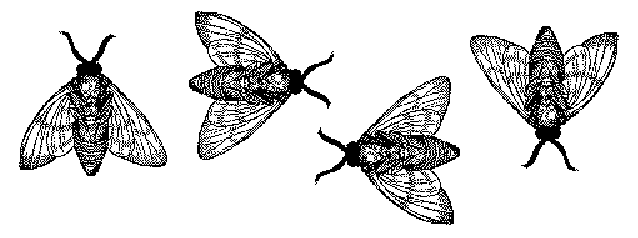
\includegraphics{flies}
% %\caption{A sample black and white graphic
% %that needs to span two columns of text.}
% %\end{figure*}


% %\begin{figure}
% %
\includegraphics[height=1in, width=1in]{rosette}
% %\caption{A sample black and white graphic that has
% %been resized with the \texttt{includegraphics} command.}
% %\end{figure}

% \subsection{Theorem-like Constructs}

% Other common constructs that may occur in your article are the forms
% for logical constructs like theorems, axioms, corollaries and proofs.
% ACM uses two types of these constructs:  theorem-like and
% definition-like.

% Here is a theorem:
% \begin{theorem}
%   Let $f$ be continuous on $[a,b]$.  If $G$ is
%   an antiderivative for $f$ on $[a,b]$, then
%   \begin{displaymath}
%     \int^b_af(t)\,dt = G(b) - G(a).
%   \end{displaymath}
% \end{theorem}

% Here is a definition:
% \begin{definition}
%   If $z$ is irrational, then by $e^z$ we mean the
%   unique number that has
%   logarithm $z$:
%   \begin{displaymath}
%     \log e^z = z.
%   \end{displaymath}
% \end{definition}

% The pre-defined theorem-like constructs are \textbf{theorem},
% \textbf{conjecture}, \textbf{proposition}, \textbf{lemma} and
% \textbf{corollary}.  The pre-defined de\-fi\-ni\-ti\-on-like constructs are
% \textbf{example} and \textbf{definition}.  You can add your own
% constructs using the \textsl{amsthm} interface~\cite{Amsthm15}.  The
% styles used in the \verb|\theoremstyle| command are \textbf{acmplain}
% and \textbf{acmdefinition}.

% Another construct is \textbf{proof}, for example,

% \begin{proof}
%   Suppose on the contrary there exists a real number $L$ such that
%   \begin{displaymath}
%     \lim_{x\rightarrow\infty} \frac{f(x)}{g(x)} = L.
%   \end{displaymath}
%   Then
%   \begin{displaymath}
%     l=\lim_{x\rightarrow c} f(x)
%     = \lim_{x\rightarrow c}
%     \left[ g{x} \cdot \frac{f(x)}{g(x)} \right ]
%     = \lim_{x\rightarrow c} g(x) \cdot \lim_{x\rightarrow c}
%     \frac{f(x)}{g(x)} = 0\cdot L = 0,
%   \end{displaymath}
%   which contradicts our assumption that $l\neq 0$.
% \end{proof}

% \section{Conclusions}
% This paragraph will end the body of this sample document.
% Remember that you might still have Acknowledgments or
% Appendices; brief samples of these
% follow.  There is still the Bibliography to deal with; and
% we will make a disclaimer about that here: with the exception
% of the reference to the \LaTeX\ book, the citations in
% this paper are to articles which have nothing to
% do with the present subject and are used as
% examples only.
% %\end{document}  % This is where a 'short' article might terminate



% \appendix
% %Appendix A
% \section{Headings in Appendices}
% The rules about hierarchical headings discussed above for
% the body of the article are different in the appendices.
% In the \textbf{appendix} environment, the command
% \textbf{section} is used to
% indicate the start of each Appendix, with alphabetic order
% designation (i.e., the first is A, the second B, etc.) and
% a title (if you include one).  So, if you need
% hierarchical structure
% \textit{within} an Appendix, start with \textbf{subsection} as the
% highest level. Here is an outline of the body of this
% document in Appendix-appropriate form:
% \subsection{Introduction}
% \subsection{The Body of the Paper}
% \subsubsection{Type Changes and  Special Characters}
% \subsubsection{Math Equations}
% \paragraph{Inline (In-text) Equations}
% \paragraph{Display Equations}
% \subsubsection{Citations}
% \subsubsection{Tables}
% \subsubsection{Figures}
% \subsubsection{Theorem-like Constructs}
% \subsubsection*{A Caveat for the \TeX\ Expert}
% \subsection{Conclusions}
% \subsection{References}
% Generated by bibtex from your \texttt{.bib} file.  Run latex,
% then bibtex, then latex twice (to resolve references)
% to create the \texttt{.bbl} file.  Insert that \texttt{.bbl}
% file into the \texttt{.tex} source file and comment out
% the command \texttt{{\char'134}thebibliography}.
% % This next section command marks the start of
% % Appendix B, and does not continue the present hierarchy
% \section{More Help for the Hardy}

% Of course, reading the source code is always useful.  The file
% \path{acmart.pdf} contains both the user guide and the commented
% code.



\bibliographystyle{ACM-Reference-Format}
\bibliography{Zotero} 

\end{document}
